% =====================================================================
% Capitolo 1 RIORDINATO — 2026-09-05
%
% NON sostituisce Cap1.tex: e' una proposta da confrontare.
%
% Il testo e' quello della candidata, spostato per seguire la catena
% logica concordata:
%
%   carenza di personale + piu' anziani
%     -> la caduta e' l'evento avverso che pesa di piu'
%     -> il costo non e' solo clinico: avvia il passaggio a vita assistita
%     -> servono quattro condizioni insieme (tempi, falsi allarmi,
%        riservatezza, costo)
%     -> quindi un dispositivo edge, vendibile in ospedale e in RSA
%        e soprattutto in casa, dove si cade di piu' e dove nessuno guarda
%     -> due domande: ci sta su cento euro? e che cosa conta davvero?
%
% I blocchi marcati [NUOVO] non erano nel testo originale.
% I blocchi marcati [VERIFICA] contengono un dato da controllare
% sulla fonte primaria prima della consegna.
% =====================================================================. 

\chapter{Contesto applicativo e definizione del problema}
\label{cap:contesto}

% [NUOVO] — sostituisce i quattro paragrafi di apertura precedenti.
% Il vecchio incipit («una delle problematiche centrali») e la mappa del
% capitolo che annunciava tre sezioni su cinque sono stati tolti.

L'Italia si conferma il paese più vecchio d'Europa e il secondo al mondo dopo
il Giappone: la popolazione anziana continua a crescere, e con essa la
domanda di assistenza. A questa tendenza se ne contrappone però una di segno
opposto, quella del personale infermieristico, il cui rapporto con la
popolazione resta inferiore alla media europea e per il quale, fra il 2026 e
il 2035, sono attesi circa ottantamila pensionamenti~\cite{fnopi}.

Fra gli eventi che rendono necessaria quell'assistenza, la caduta occupa un
posto particolare. Può provocare conseguenze fisiche anche gravi e, al tempo
stesso, compromettere l'autonomia della persona: incide quindi sia sulla
salute sia sulla possibilità di continuare a vivere in modo indipendente.

Le conseguenze economiche seguono su due fronti. In ospedale e nelle
Residenze Sanitarie Assistenziali una caduta si traduce in giornate di
degenza, in un percorso di riabilitazione e in un fabbisogno di personale che
è proprio ciò che scarseggia. Al domicilio il carico ricade invece sulle
famiglie: in Italia circa 1,1 milioni di persone svolgono un ruolo di
assistenza informale, spesso sostenendo di tasca propria le spese
corrispondenti~\cite{fnopi}. E non tutti hanno una famiglia su cui contare.

In questo scenario si inseriscono i sistemi di \emph{fall detection},
progettati con l'obiettivo di monitorare in modo continuo il comportamento
della persona, riconoscere tempestivamente una possibile caduta e generare
una segnalazione di allarme. Costituiscono una delle applicazioni centrali
dell'\emph{Ambient Assisted Living} (AAL)~\cite{aal}, il campo che studia
l'impiego delle tecnologie dell'informazione a sostegno dell'autonomia delle
persone anziane o fragili.

Useremo questo primo capitolo per fornire una breve introduzione al contesto
nel quale un sistema di rilevamento deve funzionare. In particolare, ci
soffermeremo sulla rilevanza delle cadute nella popolazione anziana e
nell'ambiente domestico; individueremo i principali requisiti che un sistema
automatico dovrebbe soddisfare; analizzeremo le difficoltà che emergono nel
passaggio da dati raccolti in condizioni controllate a un ambiente reale; e
mostreremo infine che «riconoscere una caduta» non individua un compito solo,
da cui discendono gli obiettivi del lavoro.

\section{Ambient Assisted Living e rilevanza clinica delle cadute}

Il progressivo invecchiamento della popolazione aumenta la necessità di
soluzioni in grado di supportare il monitoraggio e l'assistenza di persone
anziane, sia in ambiente domestico sia in contesti assistenziali come
strutture ospedaliere e Residenze Sanitarie Assistenziali (RSA).

Al 1º gennaio 2026, secondo il Rapporto annuale ISTAT, le persone di età pari
o superiore a 65 anni rappresentano il 25,1\% della popolazione italiana. È
una fascia in crescita: nell'arco di un decennio è aumentata dell'11,3\%,
mentre nello stesso periodo la popolazione fino ai 14 anni è diminuita
(Figura~\ref{fig:popolazione})~\cite{istat2026}. Si tratta quindi di una
fascia numericamente rilevante, destinata ad avere un peso sempre maggiore
sui servizi sanitari, assistenziali e domiciliari.

\begin{figure}[htbp]
    \centering
    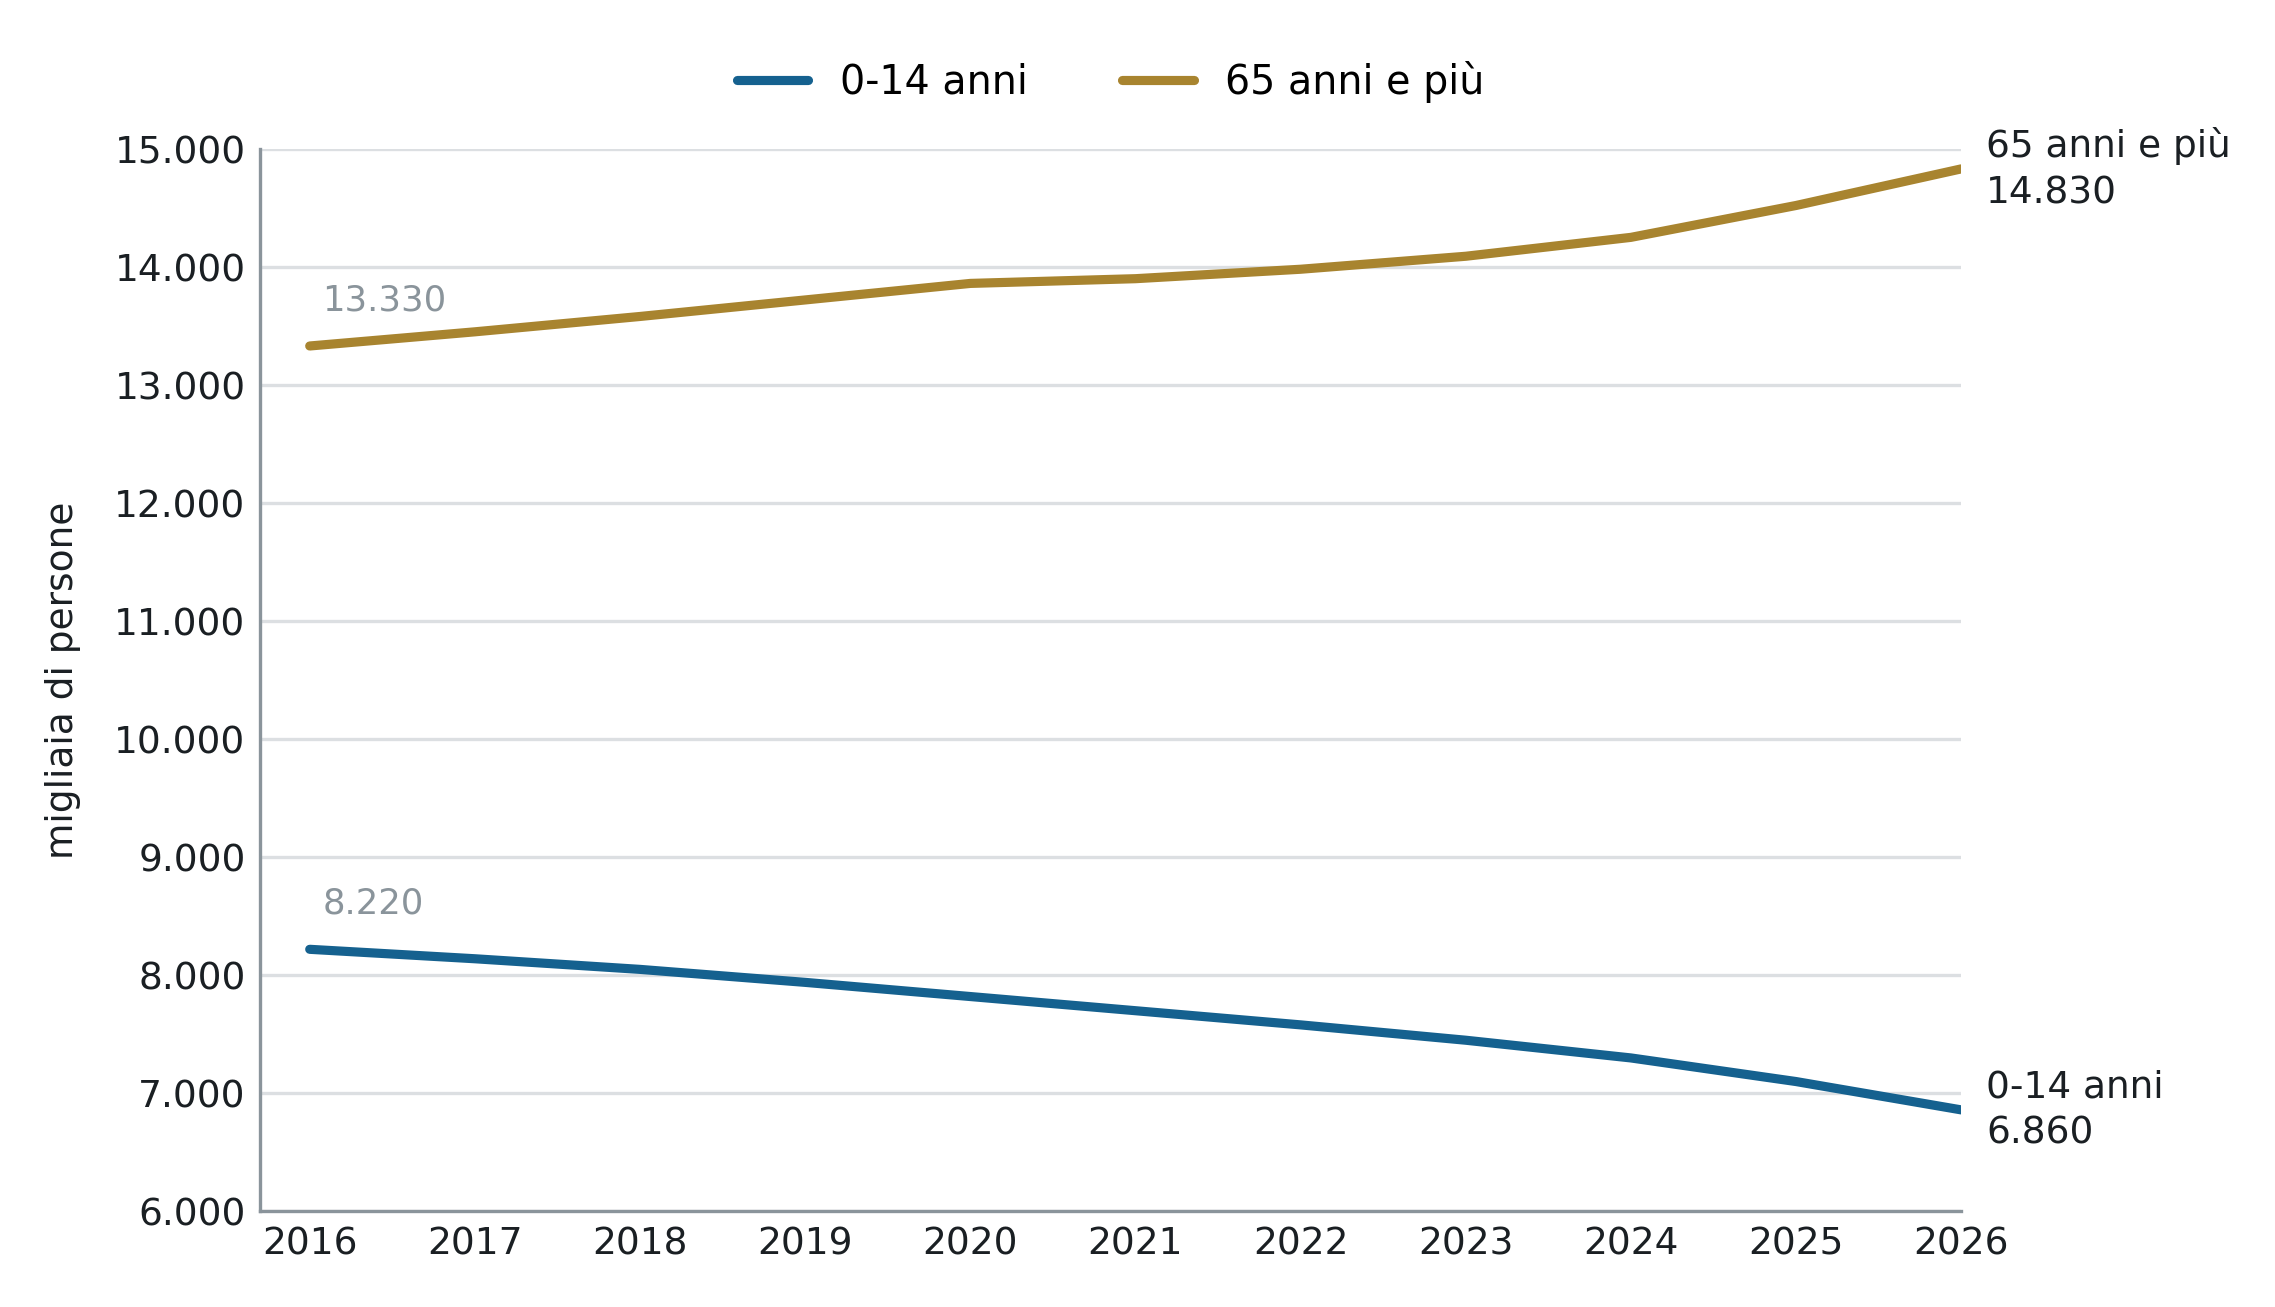
\includegraphics[width=0.82\linewidth]{figure/fig_popolazione.png}
    \caption{Popolazione italiana nelle fasce di età 0--14 e 65 anni e più,
    2016--2026, valori assoluti in migliaia. Elaborazione su dati
    ISTAT~\cite{istat2026}.}
    \label{fig:popolazione}
\end{figure}

All'interno di questa fascia di età le cadute rappresentano un evento critico
sia per frequenza sia per le conseguenze sulla salute e sull'autonomia della
persona. Secondo la sorveglianza \emph{PASSI d'Argento} dell'Istituto
Superiore di Sanità, nel biennio 2023--2024 circa un anziano su cinque
riferisce almeno una caduta nei dodici mesi precedenti. La frequenza aumenta
sensibilmente con l'età, passando dal 15\% nella fascia 65--74 anni al 31\%
oltre gli 85, ed è più elevata nelle donne, con il 24\% contro il 15\%
osservato negli uomini~\cite{passi}.

\subsection*{Cadute in ambiente domestico e conseguenze cliniche ed esistenziali}

In un sistema di rilevamento delle cadute non basta sapere quanto spesso una
persona cada: contano anche il luogo dell'evento e il tempo necessario perché
qualcuno se ne accorga.

Le cadute negli ultra sessantacinquenni avvengono prevalentemente in ambiente
domestico: circa il 54\% si verifica in casa, contro il 21\% in giardino, il
20\% in strada e il restante 5\% altrove~\cite{passi}. Casa e giardino
insieme, cioè il domicilio, rendono conto di tre cadute su quattro.

Anche in una struttura ospedaliera o assistenziale le cadute sono frequenti.
In quel contesto, però, la presenza di personale rende generalmente più
probabile che l'evento venga osservato e che il soccorso arrivi in tempi
brevi. In un'abitazione quella sorveglianza non c'è, e per chi vive solo la
stessa caduta produce un tempo a terra molto più lungo.

Il valore di un rilevamento automatico è quindi massimo dove la sorveglianza
umana è assente. Questo non esclude l'impiego in ospedale o in RSA, dove un
sistema di questo tipo resta utile per ridurre i tempi di intervento; spiega
però perché il caso domestico sia quello su cui il presente lavoro si
concentra, e quello in cui è stato validato sperimentalmente.

Le conseguenze di una caduta non dipendono soltanto dall'evento traumatico
iniziale. Nel biennio 2023--2024 il 18\% delle cadute ha causato una frattura
e il 16\% ha richiesto un ricovero ospedaliero di almeno un
giorno~\cite{passi}; fra i ricoveri per incidente domestico nella popolazione
anziana la diagnosi più frequente è la frattura del femore, che nel 2010
riguardava circa la metà dei casi~\cite{epicentro}. A questo si aggiunge il
problema della permanenza a terra, che può favorire complicanze secondarie
come disidratazione, ipotermia, danno muscolare e un peggioramento generale
delle condizioni cliniche.

% [NUOVO] — il paragrafo che il titolo della sottosezione promette
% («esistenziali») e che nella versione precedente non c'era.
A queste conseguenze se ne aggiunge una che i dati clinici non registrano.
Una caduta lascia insicurezza: il timore di cadere di nuovo riduce
l'attività, accelera il declino funzionale e può indurre isolamento, fino a
compromettere lo svolgimento delle attività quotidiane più semplici. È spesso
questo, più della frattura, ciò che avvia il passaggio a una vita assistita.

Ridurre il tempo che intercorre tra la caduta e il soccorso non serve dunque
soltanto a limitare il danno immediato: serve a rendere sostenibile la
permanenza al domicilio.

\section{Requisiti di un sistema automatico di fall detection}

Un sistema destinato al rilevamento delle cadute in ambiente domestico o
assistenziale deve soddisfare vincoli differenti rispetto a un classificatore
valutato esclusivamente su dataset offline. Non basta che il modello raggiunga
buone prestazioni di classificazione: perché il sistema venga adottato, deve
segnalare l'evento in tempi brevi, non produrre tanti falsi allarmi da essere
spento dopo una settimana, trattare i dati in modo che l'installazione sia
ammissibile in un ambiente privato, e costare poco abbastanza da poter essere
effettivamente acquistato.

Sono quattro condizioni, e si traducono in tre requisiti: le prime due ---
riconoscere l'evento in fretta e non sommergere di segnalazioni chi deve
verificarle --- non si possono trattare separatamente.

\subsection{Tempestività e sostenibilità del carico di allarmi}

Il primo requisito riguarda la tempestività. Se il danno dipende anche dal
tempo trascorso a terra, come discusso nella sezione precedente, il sistema
deve riconoscere l'evento e generare una segnalazione in un intervallo
sufficientemente breve da rendere possibile una richiesta di assistenza.

La tempestività non può però essere considerata separatamente
dall'affidabilità dell'allarme. Un sistema continuamente attivo produce
infatti un numero elevato di decisioni e ogni falso positivo può richiedere
una verifica da parte di un familiare, di un caregiver o del personale
assistenziale. Se queste segnalazioni diventano troppo frequenti, il sistema
rischia di risultare poco utile nell'utilizzo quotidiano, anche nel caso in
cui riesca a riconoscere correttamente la maggior parte delle cadute.

Nei sistemi utilizzati in condizioni reali assume quindi particolare
importanza il numero di falsi allarmi prodotti per unità di tempo. Kangas et
al.\ hanno valutato un sistema di fall detection durante circa 15\,500 ore di
funzionamento, riportando un tasso di falsi allarmi pari a 0,049
allarmi/ora, successivamente ridotto a 0,025 allarmi/ora mediante una
modifica dell'algoritmo~\cite{kangas}. Analogamente, il sistema AIDE-MOI
documenta come la via seguita per ridurre le segnalazioni errate durante il
funzionamento reale sia stato un intervento sulla logica di rilevamento, e
non sul classificatore~\cite{aidemoi}.

Nel presente lavoro il sistema viene quindi valutato su due livelli distinti:
le prestazioni del classificatore sulle singole finestre temporali, e il
numero di eventi di allarme effettivamente generati durante un funzionamento
prolungato. Sono due grandezze diverse, e il Capitolo~\ref{cap:campo} mostra
di quanto differiscano.

\subsection{Riservatezza e trattamento locale delle immagini}

% [NUOVO] — la sottosezione era impostata come scelta tecnica («riduce la
% dimensionalita' dei dati»). Qui diventa una condizione di ammissibilita',
% che e' il ruolo che ha davvero nel lavoro.

L'utilizzo di una telecamera all'interno di un'abitazione o di una struttura
assistenziale introduce un secondo requisito, che non è tecnico ma di
ammissibilità. Un flusso RGB contiene informazioni identificative sulla
persona, sull'ambiente in cui vive e sulle attività che sta svolgendo; e le
cadute avvengono anche negli ambienti in cui l'aspettativa di riservatezza è
più alta --- il bagno, la camera da letto --- che sono proprio quelli in cui
una telecamera tradizionale non è installabile.

% [VERIFICA] — impianto giuridico: GDPR artt. 5(1)(c), 25 e 35, e Linee guida
% EDPB 3/2019 sui dispositivi video. Far controllare a chi ha competenza.
Il Regolamento europeo sulla protezione dei dati non vieta il trattamento, ma
impone che i dati trattati siano adeguati, pertinenti e limitati a quanto
necessario rispetto alla finalità perseguita. La finalità, qui, è riconoscere
una caduta: se per riconoscerla è sufficiente la configurazione geometrica del
corpo, trasmettere o conservare l'immagine eccede quanto necessario. Il
criterio non è quindi se il trattamento sia lecito, ma se esista un modo meno
invasivo di ottenere lo stesso risultato.

Nel presente lavoro il video viene perciò impiegato soltanto nella prima fase
della pipeline, nella quale viene stimata la posa del soggetto mediante
MediaPipe Pose~\cite{mediapipe}, costruito sull'architettura
BlazePose~\cite{blazepose}. Da ciascun frame vengono estratti i principali
\emph{landmark} del corpo, dai quali vengono poi costruite le feature
geometriche e temporali utilizzate per la classificazione.

La minimizzazione non è una configurazione del sistema, ma una proprietà
della sua architettura: il fotogramma viene scartato subito dopo la stima
della posa, e volto, texture, abbigliamento e sfondo non raggiungono le fasi
successive. Ne segue che il modello \emph{non può} apprendere l'aspetto delle
persone osservate al posto del loro movimento. L'ingresso del classificatore
è una rappresentazione numerica della configurazione e della dinamica del
corpo, e l'elaborazione avviene interamente sul dispositivo: verso l'esterno
vengono trasmessi soltanto i dati necessari alla gestione di un eventuale
allarme.

È questa proprietà a rendere il sistema installabile dove un dispositivo
basato su immagini non lo sarebbe, ed è ciò che lo distingue sia dai sistemi
che affidano l'elaborazione a un servizio remoto, sia dai dispositivi
indossabili, la cui efficacia dipende dal fatto che la persona li indossi.

\subsection{Costo, risorse e architettura edge}

La scelta di eseguire localmente l'elaborazione introduce un vincolo sulle
risorse computazionali disponibili. Un sistema destinato a essere installato
in modo continuativo in un'abitazione o in una struttura assistenziale
dovrebbe poter funzionare su hardware compatto e a basso costo, senza
dipendere da una workstation o da un'infrastruttura di calcolo remota. Il
lavoro adotta quindi un'architettura \emph{edge}, nella quale l'acquisizione
del video, la stima della posa, la costruzione delle feature e la
classificazione vengono eseguite direttamente sul dispositivo.

Il problema non consiste dunque soltanto nel massimizzare le prestazioni del
classificatore: occorre trovare un compromesso fra capacità di
riconoscimento, complessità computazionale, latenza e possibilità di
mantenere l'intera pipeline attiva nel tempo.

Il costo computazionale va inoltre considerato sull'intera catena di
elaborazione. Prima di ottenere una decisione è necessario acquisire il
frame, stimare la posa della persona, calcolare le feature che descrivono il
movimento e infine applicare il classificatore. La fattibilità sul
dispositivo \emph{edge} deve quindi essere verificata su tutte queste fasi, e
non soltanto sul modello che produce la decisione finale.

\section{Criticità del trasferimento dal dato controllato all'ambiente reale}

La valutazione su un dataset controllato permette di confrontare in modo
riproducibile rappresentazioni e modelli, ma non garantisce che il sistema
mantenga lo stesso comportamento una volta installato in un ambiente reale.

Durante la raccolta di un dataset molte condizioni sono infatti note o
controllate: la posizione delle telecamere, le attività eseguite dai
soggetti, la durata delle registrazioni e, in generale, il contesto nel quale
avviene l'acquisizione. In un'abitazione reale queste condizioni possono
invece variare nel tempo.

Nel caso di un sistema basato sulla stima della posa, tre aspetti sono
particolarmente importanti: il cambiamento del dominio e della geometria di
ripresa, la presenza di occlusioni e la diversa frequenza con cui una caduta
si presenta rispetto alle normali attività quotidiane.

\subsection{Variazione del dominio e geometria di ripresa}

Una prima criticità è rappresentata dal cambiamento delle condizioni di
acquisizione. La rappresentazione ottenuta dallo stimatore di posa dipende
infatti non soltanto dal movimento eseguito dalla persona, ma anche dal modo
in cui questo movimento viene osservato dalla telecamera.

Una stessa azione può apparire differente se osservata frontalmente,
lateralmente o da una posizione più elevata. Di conseguenza, anche grandezze
ricavate dai landmark, come l'inclinazione del tronco, gli spostamenti delle
diverse parti del corpo o le loro velocità apparenti, possono assumere valori
differenti pur descrivendo lo stesso movimento.

% Il paragrafo «Il cambiamento del punto di vista rappresenta quindi un
% problema importante...» e' stato tolto: ripeteva quello sopra.

A questo si aggiungono altre variazioni, come l'illuminazione, la distanza
dalla telecamera, lo sfondo, il frame rate e le caratteristiche fisiche dei
soggetti osservati. Nel loro insieme, queste differenze determinano un
\emph{domain shift}, cioè una variazione della distribuzione dei dati
rispetto a quella utilizzata durante l'addestramento.

Le prestazioni ottenute sul dominio di partenza non bastano quindi, da sole,
a descrivere la capacità di generalizzazione del sistema. Nel seguito viene
perciò considerato anche il comportamento della rappresentazione quando
cambiano il punto di vista e il dataset utilizzato per la valutazione.

\subsection{Occlusioni e qualità della stima della posa}

Una seconda criticità riguarda la visibilità del corpo. Nei dataset raccolti
in condizioni controllate il soggetto è generalmente ripreso in modo da
risultare ben visibile. In un ambiente domestico o assistenziale, invece, la
persona può essere parzialmente nascosta da letti, sedie, tavoli o altri
elementi dell'arredamento. L'occlusione può inoltre verificarsi proprio
durante una caduta, quando il corpo cambia rapidamente configurazione o si
avvicina al pavimento.

In tali condizioni lo stimatore di posa può fornire coordinate instabili o
non riuscire a localizzare correttamente alcuni landmark. Il problema è
particolarmente importante nel presente lavoro, perché le feature utilizzate
dal classificatore vengono costruite proprio a partire dalle coordinate dello
scheletro: un errore nella stima di un landmark può propagarsi alle grandezze
geometriche e temporali calcolate nelle fasi successive.

Il sistema deve essere valutato tenendo conto anche di questa sorgente di
errore. Nel Capitolo~\ref{cap:protocollo} la sensibilità a una perdita
parziale dell'informazione viene studiata attraverso prove controllate nelle
quali alcuni gruppi di landmark vengono resi temporaneamente non disponibili.

\subsection{Prevalenza dell'evento e frequenza di base dei falsi allarmi}

Un'ulteriore differenza fra un dataset sperimentale e il funzionamento reale
riguarda la \textbf{prevalenza della classe positiva}, cioè la frequenza con
cui si verificano realmente le cadute.

Per costruire un dataset utile all'addestramento è necessario includere un
numero sufficiente di esempi positivi. La proporzione di cadute presente nei
dati sperimentali è quindi molto maggiore di quella che un sistema incontra
durante un funzionamento continuo, nel quale la grande maggioranza delle
osservazioni appartiene alle normali attività quotidiane. È un fatto che
modifica in modo importante l'interpretazione dei falsi positivi.

Si consideri, ad esempio, un sistema che produce $4{,}5$ decisioni al
secondo. Nell'arco di un anno il numero complessivo di decisioni sarebbe
circa
\[
4{,}5 \cdot 60 \cdot 60 \cdot 24 \cdot 365 \simeq 1{,}42 \cdot 10^{8}.
\]
Supponendo un tasso di falsi positivi pari allo $0{,}01\%$, apparentemente
molto basso, si otterrebbero comunque
\[
1{,}42 \cdot 10^{8} \cdot 10^{-4} \simeq 1{,}42 \cdot 10^{4}
\]
decisioni positive errate all'anno. L'esempio mostra come un errore poco
rilevante sulla singola decisione possa diventare problematico quando il
sistema rimane attivo per periodi molto lunghi.

È però necessario distinguere le predizioni prodotte dal classificatore dagli
allarmi effettivamente generati. Più finestre positive consecutive possono
infatti appartenere allo stesso episodio e venire aggregate dalla logica del
sistema in un unico evento. Diventa quindi utile considerare due livelli di
valutazione: il primo riguarda le singole finestre temporali e permette di
studiare il classificatore, il secondo riguarda gli eventi di allarme
prodotti durante il funzionamento continuo. Nel secondo caso la misura più
significativa è il numero di falsi allarmi per unità di tempo, perché
rappresenta direttamente il carico che il sistema impone all'utente, ai
familiari o al personale assistenziale.

\section{Definizione dell'evento da riconoscere}

Un'ultima difficoltà riguarda la definizione stessa di ciò che il sistema
deve riconoscere.

Una caduta non è infatti una singola postura, ma un evento che si evolve nel
tempo. La persona parte da una configurazione stabile, attraversa una fase di
perdita dell'equilibrio e di rapida variazione della postura, e può infine
raggiungere una configurazione a terra o comunque su un livello inferiore. È
quindi possibile distinguere una condizione precedente all'evento, una fase
di transizione durante la caduta e uno stato successivo nel quale il soggetto
rimane a terra.

Dal punto di vista della classificazione, il fenomeno può essere descritto in
modi differenti. Una prima possibilità consiste nel riconoscere l'\emph{evento
di caduta}, cioè la fase dinamica durante la quale il corpo perde l'equilibrio
e si sposta rapidamente verso il basso. Una seconda consiste nel riconoscere
lo \emph{stato successivo alla caduta}, nel quale la persona si trova già a
terra. Una terza possibilità consiste infine nel considerare rilevanti
entrambe le condizioni ai fini della generazione dell'allarme.

Queste formulazioni sono strettamente collegate, ma non sono equivalenti. Una
persona può infatti trovarsi in una posizione bassa o distesa anche durante
una normale attività quotidiana: sedersi, inginocchiarsi o sdraiarsi
volontariamente portano il corpo ad assumere configurazioni simili a quelle
osservate dopo una caduta.

% [NUOVO] — aggancio empirico che collega questa sezione alla 1.1.
Il problema non è astratto. Fra le cadute che avvengono in casa, quelle che
compaiono a partire dai sessant'anni comprendono le cadute dal letto e quelle
che avvengono alzandosi da una sedia~\cite{epicentro}: in questi casi il
corpo parte da una superficie rialzata e raggiunge una configurazione finale
molto simile a quella di chi vi si è disteso volontariamente.

La sola postura finale può quindi non bastare a distinguere una caduta da
un'attività normale. L'informazione discriminante è invece la dinamica con
cui quella postura viene raggiunta: una caduta è generalmente associata a una
variazione rapida e poco controllata della configurazione del corpo, mentre
un movimento volontario tende a presentare un'evoluzione più regolare.

La definizione della classe positiva rappresenta dunque una scelta
metodologica nella formulazione del problema, e non una semplice convenzione
di etichettatura. Cambiare ciò che viene considerato positivo significa
modificare il compito richiesto al classificatore e, di conseguenza, anche il
tipo di errori che il sistema può produrre. Nel lavoro svolto le diverse
formulazioni vengono perciò considerate separatamente, per valutarne il
comportamento sia sui dati controllati sia in condizioni più vicine a quelle
reali.

\section{Obiettivi}

Alla luce delle considerazioni precedenti, l'obiettivo di questo lavoro è
sviluppare e valutare un sistema di \emph{fall detection} basato sull'analisi
del movimento umano, progettato per essere eseguito localmente su un
dispositivo \emph{edge} a basso costo. L'idea di base consiste
nell'utilizzare il video RGB come sorgente percettiva, estrarre localmente
una rappresentazione scheletrica del soggetto e svolgere la classificazione
temporale su un insieme compatto e interpretabile di grandezze derivate dal
movimento del corpo.

% [NUOVO] — le due domande. Sostituisce «L'obiettivo non e' quindi soltanto
% ottenere buone prestazioni all'interno del dataset...», che era la terza
% occorrenza della stessa affermazione.
Il lavoro risponde a due domande distinte. La prima è di fattibilità: se
l'intera catena --- acquisizione, stima della posa, costruzione delle
feature, classificazione e logica di allarme --- possa essere eseguita in
modo continuo su un dispositivo a basso costo. La seconda riguarda ciò che
determina il comportamento del sistema: fra rappresentazione del movimento,
definizione dell'evento da riconoscere, architettura del classificatore e
protocollo di valutazione, quali di queste scelte incidono su come il sistema
si comporta in un ambiente reale, e quali invece risultano ininfluenti.

Le due domande hanno natura diversa. La prima si decide misurando sul
dispositivo, e la risposta non dipende dal numero di soggetti osservati. La
seconda si decide confrontando configurazioni, e per alcuni dei confronti il
numero di soggetti disponibile non è sufficiente a distinguerle: dichiararlo
fa parte della risposta.

Il lavoro si sviluppa lungo quattro direzioni principali:

\begin{enumerate}
    \item \textbf{Rappresentazione del movimento}: costruire, a partire dai
    landmark scheletrici, rappresentazioni geometriche e temporali compatte e
    interpretabili, in grado di descrivere l'evoluzione del corpo durante una
    caduta e durante normali attività quotidiane.

    \item \textbf{Classificazione temporale}: confrontare diverse famiglie di
    modelli applicate alla stessa rappresentazione del movimento, in modo da
    valutare quanto la scelta del classificatore influenzi le prestazioni
    rispetto alle altre componenti della pipeline.

    \item \textbf{Definizione del compito e protocollo di valutazione}:
    analizzare l'effetto delle principali scelte sperimentali, relative alla
    costruzione delle finestre temporali, all'etichettatura, alla separazione
    dei soggetti fra addestramento e test e alla definizione dell'evento da
    riconoscere.

    \item \textbf{Fattibilità e trasferibilità del sistema}: controllare che
    l'intera pipeline sia compatibile con le risorse di un dispositivo edge e
    studiarne il comportamento quando cambiano il soggetto, il punto di vista,
    il dataset e l'ambiente di acquisizione.
\end{enumerate}

Le prime tre direzioni rispondono alla seconda domanda, la quarta alla prima.
In sintesi, il sistema deve riconoscere una caduta limitando il rischio di
eventi non rilevati, senza generare al tempo stesso un numero di falsi
allarmi incompatibile con un utilizzo continuativo. La valutazione dovrà
quindi tenere conto sia delle prestazioni del classificatore sia delle
esigenze pratiche poste da un'applicazione destinata al funzionamento reale.
